\begin{frame}[fragile]
\frametitle{Basic Text Manipulation with \LaTeX{}}
    \LaTeX{} handles text manipulation and formatting differently than word processors. \\[\baselineskip] \pause
    Instead of editing the output document directly, content is written in plain text and annotated with different commands to indicate styles, sizes, placement, etc. \\[\baselineskip] \pause
    \LaTeX{} takes these commands and compiles the source code into a document. \\[\baselineskip] \pause
    This gives the author significant control over all aspects of the document. \\[\baselineskip]
\end{frame}


\begin{frame}[fragile]
\frametitle{Font Modifiers: Size}
\begin{block}{Optional Arguments in the Preamble}
    \begin{minted}{latex}
    \documentclass[10pt]{article}
    \documentclass[11pt]{article}
    \documentclass[12pt]{article}
    \end{minted}
\end{block} \pause
\begin{block}{Font Modifiers Within Body}
    \begin{columns}
    \column{0.33\textwidth}
    \begin{minted}{latex}
    \tiny
    \scriptsize
    \footnotesize
    \end{minted}
    \column{0.33\textwidth}
    \begin{minted}{latex}
    \normalsize
    \large
    \Large
    \end{minted}
    \column{0.33\textwidth}
    \begin{minted}{latex}
    \LARGE
    \huge
    \HUGE
    \end{minted}
    \end{columns}
\end{block} \pause
Font modifiers act \emph{relative} to the main document font size.
\end{frame}


\begin{frame}[fragile]
\frametitle{Font Modifiers: Size}
Font modifiers can act like a ``switch" to change the font size for all subsequent text within the document, OR font modifiers can act like a ``function" to change the font size for a limited scope. \pause
\begin{block}{Examples}
\footnotesize
\verb|Normal size \LARGE LARGE text| $\to$ Normal size {\Large LARGE text}  \\
\vspace{0.5cm}
\footnotesize
\verb|Normal size {\LARGE LARGE } text| $\to$ Normal size {\Large LARGE} text \\
\vspace{0.5cm}
\end{block} \pause
Other font size packages include: \verb|extsizes|, \verb|anyfontsize|.
\end{frame}


\begin{frame}[fragile]
\frametitle{Font Modifiers: Styles}
\textbf{Bold}, \textit{italic}, and \underline{underline} act on text delimited by \verb|{|, \verb|}|. \pause
\begin{block}{Bold, italic, underline}
    \verb|Normal text| $\to$ Normal text \\ \pause
    \vspace{0.2cm}
    \verb|\textbf{Bold text}| $\to$ \textbf{Bold text} \\ \pause
    \vspace{0.2cm}
    \verb|\textit{Italic text}| $\to$ \textit{Italic text} \\ \pause
    \vspace{0.2cm}
    \verb|\underline{Underlined text}| $\to$ \underline{Underlined text} \\ \pause
\end{block}
These options can be combined. \pause
\begin{block}{Combination Examples}
    \verb|\textbf{textit{Bold italic text}}| $\to$ \textbf{\textit{Bold italic text}} \\
    \vspace{0.2cm}
    \verb|\textbf{textit{\underline{B I U text}}}| $\to$ \textbf{\textit{\underline{B I U text}}} \\
\end{block}
\end{frame}


\begin{frame}[fragile]
\frametitle{Font Modifiers: Styles}
Text emphasis is a content-driven font choice performed by \LaTeX{}. \pause
\begin{block}{Text Emphasis}
    \small
    \verb|Regular \emph{emphasis} text| $\to$ Regular \emph{emphasis} text \\
    \vspace{0.2cm}
    \verb|\textit{Italic \emph{emphasis} text}| $\to$ \textit{Italic} emphasis \textit{text} \\
    \vspace{0.2cm}
    \verb|\emph{Emphatic \emph{emphasis} text}| $\to$ \textit{Emphatic} emphasis \textit{text} \\
    \vspace{0.2cm}
\end{block} \pause
\LaTeX{} chooses the specific emphasis depending on the surrounding text.
\end{frame}


\begin{frame}[fragile]
\frametitle{Font Modifiers: Families}
There are three primary font families available: \textrm{Roman}, \textsf{Sans Serif}, and \texttt{Typewriter}. \pause
\begin{block}{Font Families}
    \verb|\textrm{Default (Roman) Text}| $\to$ \textrm{Default (Roman) Text} \\ \pause
    \vspace{0.2cm}
    \verb|\textsf{Sans Serif Text}| $\to$ \textsf{Sans Serif Text} \\ \pause
    \vspace{0.2cm}
    \verb|\texttt{Typewriter Text}| $\to$ \texttt{Typewriter Text} \\ \pause
    \vspace{0.2cm}
\end{block}
\textrm{Roman} is the default font family. \\ \pause
\texttt{Typewriter text} is a monospaced font used for code snippets (we'll get to those later).
\end{frame}


\begin{frame}[fragile]
\frametitle{Font Modifiers: Colors}
Color manipulation in a \LaTeX{} document uses the \keytt{xcolor} package. There are three additional options which provide more named colors: \pause
\begin{itemize}
    \item \keytt{dvipsnames} loads 68 named colours (CMYK)
    \item \keytt{svgnames} loads 151 named colours (RGB)
    \item \keytt{x11names} loads 317 named colours (RGB) 
\end{itemize} \pause
\begin{exampleblock}{}
\begin{minted}{latex}
\usepackage{xcolor}
\usepackage[dvipsnames]{xcolor}
\usepackage[isvgnames]{xcolor}
\usepackage[x11names]{xcolor}
\end{minted}
\end{exampleblock} \pause
It's also possible to define your own colors! \textit{(But we aren't getting into that right now...)}
\end{frame}


\begin{frame}[fragile]
\frametitle{Font Modifiers: Colors}
The \keytt{dvipsnames} option in the \keytt{xcolor} package provides the the following named colors:\\
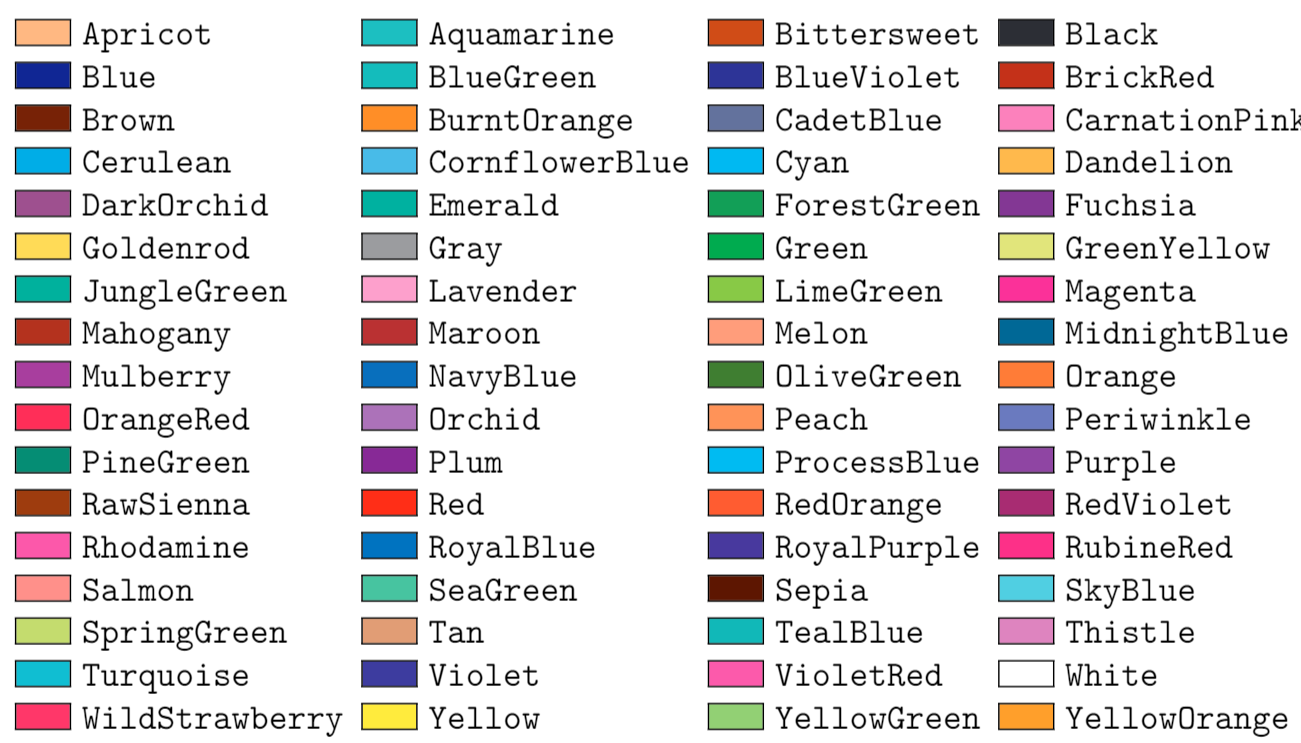
\includegraphics[width=\linewidth]{img/dvipsnamesXcolor.png}
\end{frame}


\begin{frame}[fragile]
\frametitle{Font Modifiers: Colors}
To recolor text, use the \keytt{textcolor} command. 
Its first argument is the desired color; its second is the text to be colored. 
\begin{exampleblock}{}
\begin{minted}{latex}
\textcolor{color}{text}
\end{minted}
\end{exampleblock} \pause
To highlight text in a certain color, use the \keytt{colorbox} command. 
Its first argument is the desired color; its second is the text to be highlighted.
\begin{exampleblock}{}
\begin{minted}{latex}
\colorbox{color}{text}
\end{minted}
\end{exampleblock} \pause
To color an entire page, use the \keytt{pagecolor} command. 
\begin{exampleblock}{}
\begin{minted}{latex}
\pagecolor{color}
\end{minted}
\end{exampleblock}
\end{frame}



\begin{frame}[fragile]
\frametitle{Text Alignment: Justification}
The default justification is \emph{fully justified}. Other justification options include: \pause
\begin{block}{Center Justified Text}
    \begin{minted}{latex}
    \begin{center} ... \end{center}    
    \end{minted}
\end{block} \pause
\begin{block}{Left Justified Text}
    \begin{minted}{latex}
    \begin{flushleft} ... \end{flushleft}    
    \end{minted}
\end{block} \pause
\begin{block}{Right Justified Text}
    \begin{minted}{latex}
    \begin{flushright} ... \end{flushright}    
    \end{minted}
\end{block}
\end{frame}


\begin{frame}[fragile]
\frametitle{Text Alignment: Justification}
\begin{columns} 
    \column{0.5\textwidth}
        {\centering \textbf{Fully Justified Text (Default)}}
            \fbox{\parbox{\textwidth}{\small 
            \vspace{0.35cm}
            Fully justified text is spaced out so that it stretches to fill the entire width of the page. The left and right margins are both perfectly straight.
            \vspace{0.35cm}}} \\ 
    \pause
        \vspace{0.2cm}
        {\centering \textbf{Left Justified Text}}
            \fbox{\parbox{\textwidth}{\small \begin{flushleft} Left justified text is aligned with the left margin. Spacing between words is not stretched; thus, the right margin will have a ragged edge.\end{flushleft}}}
    \pause
    \column{0.5\textwidth}
        {\centering \textbf{Center Justified Text}}
            \fbox{\parbox{\textwidth}{\small \begin{center} Center justified text is aligned down the center of the page. Spacing between words is unstretched; thus, both margins have ragged edges.\end{center}}} \\
    \pause
        \vspace{0.2cm}
        {\centering \textbf{Right Justified Text}}
            \fbox{\parbox{\textwidth}{\small \begin{flushright} Right justified text is aligned with the right margin. Spacing between words is not stretched; thus, the left margin will have a ragged edge.\end{flushright}}}
\end{columns}
\end{frame}


\begin{frame}[fragile]
\frametitle{Text Alignment: Line Breaks}
\begin{block}{Line Breaks}
    \begin{minted}{latex} 
    Here's a line of text. \\
    This is another line of text. \\[\baselineskip]
    ...And another line of text \\[2\baselineskip]
    Here's the last line of text.
    \end{minted}
\end{block}
\vspace{0.4cm}
    \fbox{\parbox{\textwidth}{Here's a line of text. \\
    This is another line of text. \\[\baselineskip]
    ...And another line of text \\[2\baselineskip]
    Here's the last line of text.}}
\end{frame}


\begin{frame}[fragile]
\frametitle{Text Alignment: Indentation}
\LaTeX{} automatically indents new paragraphs. 
\begin{itemize}
    \item[$\bullet$] To skip indentation of a single paragraph: 
    \item \verb|\noindent|
    \item[$\bullet$] To change indentation for the entire document: \verb|\setlength{\parindent}{1cm}|
\end{itemize}
\end{frame}



\begin{frame}[fragile]
\frametitle{Basic Text Manipulation: Summary}
\LaTeX{} allows you to modify... \pause
\begin{itemize}
    \item Text appearance
    \begin{itemize}
        \item Font size (as a ``function" or as a ``switch")
        \item Font style (\textbf{bold}, \textit{italic}, \underline{underline}, \emph{emphasis})
        \item Font family (\textrm{Roman}, \textsf{Sans Serif}, \texttt{Typewriter})
    \end{itemize} \pause
    \item Text alignment
    \begin{itemize}
        \item Justification (left, right, center, fully justified)
        \item Line breaks (single or multiple lines)
        \item Indentation \small (\verb|\noindent| or \verb|\setlength{\parindent}{...}|
    \end{itemize} \pause
\end{itemize}
... and more!
\end{frame}
